%%
%% {{{1 Title + Outline
\begin{frame}
\titlepage
Supervisor: O. Sauter
\hfill
Expert: S. Nowak
\end{frame}
%%
\begin{frame}{\vspace{5mm}\hspace{14mm} Outline}
%\begin{center}
%\LARGE Outline
%\end{center}
\tableofcontents
\end{frame}
%% }}}1
%% {{{1 Intro
\section{Introduction}
\begin{frame}
Introduction
\begin{itemize}[<+->]
	\item ITER
	\item Reference scenario: ELMy H-mode
	\item Need to understand better the physics of the H-mode
	\item Transport in between ELMs
\end{itemize}
\end{frame}
\note{\justifying%
The next step in fusion research is ITER.
		
Its reference scenario will be an ELMy H-mode. This regime is not yet fully understood, and we need a better knowledge of it to be able to use it safely and fully.

We need to understand the physics of the H-mode.

In this work we have studied the profiles evolution and the ELM effects in the inter-ELM phase.
}
%% }}}1
%% {{{1 ELMs
\section{ELMs}
\begin{frame}
ELMs
\begin{itemize}[<+->]
	\item Periodically expel particles and energy
	\item Combination of MHD modes~\cite{loennroth2004}:
	\begin{itemize}[<+->]
		\item ballooning modes ($\alpha = - R_0 q^2 \ddsd{\beta}{r}$)
		\item external kink ($j_{\Par,a} / \avg{j_{\Par}}$)
	\end{itemize}
	\item Stability given by $j - \alpha$ diagram
\end{itemize}
\end{frame}
\note{\justifying%
ELMs expel some particles and energy. This is useful to avoid the density getting too high and to clean the plasma by getting rid of impurities. But they can cause destructive erosion of the device, which could make the latter not viable.

They are an MHD instability.

They are believed to be a combination of the ballooning modes and the external kink~\cite{loennroth2004}. The ballooning mode stability parameter is the normalized pressure gradient whereas the external kink uses the normalized toroidal edge current density.

The stability of the ELM is described by the diagram of $j - \alpha$ for a given location in the pedestal.
}
%% }}}1
%% {{{1 Implementation
\section{Implementation}
\begin{frame}
Implementation of the H-mode
\begin{itemize}
	\item H-mode $\chi_e$
\end{itemize}
\end{frame}
\note{\justifying%
The implementation of transport simulations requires the electron thermal diffusivity, which is not measured in TCV. We have some scripts that compute its profile, but they strongly depend on the measurements of the density and of the temperature because of the sharp gradients found in the edge. Since these are not precisely enough measured, the electron thermal diffusivity is also not available from scripts for H-mode, thus we have to build it ourselves.
}
\begin{frame}
\begin{center}
\only<1|handout:0>{\includegraphics[height=6cm]{../matlab/pics/a_he_1.eps}}
\only<2|handout:0>{\includegraphics[height=6cm]{../matlab/pics/a_he_1bis.eps}}
\only<3|handout:0>{\includegraphics[height=6cm]{../matlab/pics/a_he_2.eps}}
\only<4>{\includegraphics[height=6cm]{../matlab/pics/a_he_3.eps}}
\end{center}
\Blue{---} L-mode $\chi_e$, \only<2|handout:0>{\Magenta{---} truncated}\only<3->{\Red{---} exp decay}, \only<4>{\Magenta{---} H-mode $\chi_e$}
\end{frame}
\note{\justifying%
We take an L-mode profile, i.e. a parabolic one.

We truncate it at the edge to create a transport barrier.

To prevent singularities to arise from this sharp cut, we use an exponential decay.

This yields the H-mode $\chi_e$ we use in our simulations.
}
\begin{frame}
Implementation of the H-mode
\begin{itemize}
	\item<1-> H-mode $\chi_e$
	\item<1-> Core $\chi_e$ scaled with $\tau_{\textrm{IPB}98(y,2)}$
	\item<2-> Pedestal $\chi_e$ scaled with $W_{\textrm{core}} \simeq 3.5 W_{\textrm{ped}}$~\cite{andreas2010}
	\item<3-> Equilibrium density computed using $\nabla n_e / n_e = V_n / D_n$ \uncover<4->{$\Longrightarrow V_n = b \cdot D_n$}
	\item<5-> Density pedestal scaled with $\nabla n_e / n_e \simeq 0.5\ \nabla T_e / T_e$~\cite{fable2006,neuhauser2002}
\end{itemize}
\end{frame}
\note{\justifying%
To ensure this profile to be as good as we can, we scale the core profile with the scaling energy confinement time.

The pedestal $\chi_e$ is scaled using a result from a recent work (APi thesis~\cite{andreas2010}) between the core and pedestal energies.

The density is also computed by the code. We implement it to match the experimental profile at the equilibrium, using this formula. Thus we set these constants to fix the ratio.

We use a scaling for the pedestal density linking it to the pedestal temperature. This scaling was found to be good in electron internal transport barriers~\cite{fable2006} and in ASDEX Upgrade H-mode pedestals~\cite{neuhauser2002}.
}
\begin{frame}
Implementation of the ELMs
\begin{itemize}
	\item<1-> Not triggered by MHD parameters
	\item<2-> ELM period: $20 ms$ (experimental data)
	\item<2-> ELM duration: $100 \mu s$ (experimental data)
	\item<3-> Acting on diffusivities
	\item<4-> Setting a high value for edge $\chi_e$, $\chi_i$ and $D_n$
	\item<5-> ELM region similar to pedestal ($\sim 0.78 < \rho_V < 1$)
\end{itemize}
\end{frame}
\note{\justifying%
The ELMs in our simulations are independent of the MHD limits, but we fix their
		
period and duration from experimental data.

To mimic an edge instability, we act on the particle and thermal diffusivities.

We set their edge to be very high whilst their core remain the same.

The ELM interaction range is set to be approximately equal to the pedestal width.
}
\begin{frame}
ELM thermal diffusivity
\begin{center}
\includegraphics[width=5cm]{../matlab/pics/a_he_ELM.eps}
\hspace{5mm}
\includegraphics[width=5cm]{../matlab/pics/40080_0.8_chie_trace.eps}
\end{center}
\end{frame}
\note{\justifying%
Here are the profile and the time trace of the $\chi_e$ used to mimic an ELM. The ion thermal diffusivity was modified exactly the same. The particle diffusivity too, but it was raised less. It was experimentally observed that the temperature pedestal flattens, but the density pedestal crashes slower. However, the value to set the $D_n^{\textrm{ELM}}$ was chosen arbitrarily and it may be better to find another value more scientifically.
}
%% }}}1
%% {{{1 H-mode simulations
\section{Simulations}
\begin{frame}
Experimental data taken as input
\begin{center}
\includegraphics[height=4cm]{../matlab/pics/40080.eps}
\hspace{15mm}
\includegraphics[height=4cm]{../matlab/pics/40080_0.8_ECHprofile.eps}
\end{center}
TCV \# 40080, $t = 0.8s$
\end{frame}
\note{\justifying%
Here is a poloidal section and the electron cyclotron (EC) heating profile of the experimental data used as input in our simulations.
}
\begin{frame}
\Blue{---} simulation data, \Red{-- --} experimental data
\begin{center}
\includegraphics[width=4cm,height=3.19cm]{../matlab/pics/40080_0.8_te_equil.eps}
\hspace{50sp}
\includegraphics[width=4cm,height=3.19cm]{../matlab/pics/40080_0.8_ne_equil.eps}\\[1mm]
\includegraphics[width=4.7cm]{../matlab/pics/40080_0.8_TIEB.eps}
\end{center}
\end{frame}
\note{\justifying%
The temperatures are presented here together with the density from the steady-state simulation (solid blue) compared to the experimental data (dashed red).

The electron temperature shows a good agreement with the experimental data except in the very center. This might be because a sawtooth crash occurred just before the measurements, explaining also the difference in the core density.

Except this, the simulated electron temperature in the core, which used the scaling energy confinement time, is not far from the experimental one. The pedestal electron temperature is computed using the energy ratio scaling. It agrees well enough with the experimental data.

The density pedestal is scaled using the link between the density gradient length and the temperature one, and it matches the experimental data very good.
}
\note{\justifying%
The fact that we have in the pedestal a scaling linking the density to the temperature and another computing the temperature using a ratio on the energy with these results gives us good confidence in both scalings.

We can make a note about the ion temperature profile. It was not of particular interest in this work, but still in the scope since ions are only heated by heat transport from the electrons. This yields a heat sink for the electrons and it must be as real as possible to be accurate.

Here is presented in red the ion temperature profile for the shot considered reconstructed from CXRS data. This shot being in the upper half of the vessel, there are not very much measurements available and the core profile has a large uncertainty. The profile in blue is the one we used in our simulations, giving as input the boundary value and setting the initial condition to be the experimental fitted profile. The pedestal values are well in the experimental data, but the core value is lower than the fitted profile.
}
\note{\justifying%
In black is shown the profile from a simulation with different settings. Andreas~\cite{andreas2010} reported that in TCV SN H-mode we have approximately $T_i \simeq T_e$ for $\rho_{\psi} > 0.85$. We have thus tried a simulation where we set both temperatures to be equal at the boundary, and also the ion thermal diffusivity equal to the electron one to create an ion temperature pedestal. This is not optimal but it was done to test the accuracy of such a profile without spending too much time.

This curve is closer to the fitted profile than the one we used. However, the pedestal seems worse in this case. For $0.8 < \rho_{\psi} < 0.9$ we have a good agreement, but further in the edge the data are not decreasing. This might be due to ELMs occurring during the measurements.
}
%% }}}1
%% {{{1 ELMy H-mode simulations (std)
\subsection{ELMy H-mode}
\begin{frame}
Temperature and density profiles through an ELM cycle
\begin{center}
\includegraphics[width=5.7cm]{../matlab/pics/40080_0.8_te_rhosOK_stdNoST.eps}
\hspace{-15mm}
\includegraphics[width=5.7cm]{../matlab/pics/40080_0.8_ne_rhosOK_stdNoST.eps}
\end{center}
\end{frame}
\note{\justifying%
Now we set some ELMs in our simulation and we are interested in their effects on the plasma.

We have the top of the temperature and density pedestal. The ELM interaction range goes to here, which is the top of the temperature pedestal. I reported using rather the top of the density pedestal, thus I must have confused myself in my report. Nevertheless, the observed coordinate is really the top of the density pedestal.

Our ELM model affects only the edge of the plasma. Andreas~\cite{andreas2010} reported that the central temperature also drops instantaneously at the ELM crash. This means that this model is not completely accurate. There are several ways to understand how to correct it.

It could be the MHD mode that is more global than thought, acting to the $q = 1$ radius ($\rho_V \simeq 0.5$ in our case), or even further since H-mode plasmas have large value of $r_1$.
}
\note{\justifying%
Another possibility is that there are global confinement effects during the ELM that make the instability able to act on the whole plasma.

A last case considered is that there is a cascading phenomenon. If we recall of the ballooning stability criterion, it depends on the pressure gradient. Our crash (in red) makes a high pressure gradient at the edge of the region affected by our ELM. Hence it is possible that it triggers another ballooning mode and so on until the center of the plasma.
}
\blanknote
\begin{frame}
Temperature ELM cycle
\begin{center}
\includegraphics[width=5cm]{../matlab/pics/40080_0.8_te_rhosOK_stdNoST.eps}
\hspace{1mm}
\includegraphics[width=5cm]{../matlab/pics/40080_0.8_te_results_cycle.eps}
\end{center}
\begin{flushright}
\Blue{---} top of $n_e$ ped, \Red{-- --} maximum of $\nabla p_e$\\
$- \cdot -$ (black) top of $T_e$ ped
\end{flushright}
\end{frame}
\note{\justifying%
Here is the temperature time traces together with its profiles. This figure in my report has the time traces of dash-dotted black and of dashed red mixed. Here it is corrected.

I reported the change in behavior in the temperature time traces depending on the location. However, I had to rerun my simulations near the end of my report and it changed this behavior without I noticed it in time. The reported change is not quite significant, and if there is a change it is rather the recovery time at the top of the temperature pedestal that is shorter than that at the maximum of the pressure gradient.

The recovery has also been experimentally observed to be very fast, around $0.3 ms$~\cite{andreas2010}, which is ten times faster than what we have with our model. This might be due to some global effects that act still after the ELM.

At the top of pedestal, the temperature drop is about $0.4 keV$. \cite{andreas2010}~reported a drop around $0.2 keV$, but the height of the pedestal was $0.4 keV$ lower than in our case.
}
\begin{frame}
Density ELM cycle
\begin{center}
\includegraphics[width=5cm]{../matlab/pics/40080_0.8_ne_rhosOK_stdNoST.eps}
\hspace{1mm}
\includegraphics[width=5cm]{../matlab/pics/40080_0.8_ne_results_cycle.eps}
\end{center}
\begin{flushright}
\Blue{---} top of $n_e$ ped, \Red{-- --} maximum of $\nabla p_e$
\end{flushright}
\end{frame}
\note{\justifying%
The density time trace at the top of pedestal exhibits a large decrease \textbf{after} the crash to refill the pedestal. Thus at this location we do not properly have a recovery time since the loss was not caused by the ELM.

The drop of density at the maximum of the pressure gradient is about $2 \cdot 10^{19} m^{-3}$. Experimental observations at the top of pedestal give rather $1 \cdot 10^{19} m^{-3}$ \cite{andreas2010}, but we have here the density height of pedestal $1.5 \cdot 10^{19} m^{-3}$ higher than the experiment. The recovery time has also been observed to be much faster in experiments ($\sim 1ms$) than in our simulations (around $10ms$).
}
\begin{frame}
\begin{center}
\includegraphics[height=6cm,width=10cm]{../matlab/pics/40080_0.8_jalpha_stdNoST.eps}
\end{center}
$\cdots$ 0 - 0.1 (crash), $- \cdot -$ 0.1 - 0.5, --- 0.5 - 1, -- -- 1 - 20 [ms]
\end{frame}
\note{\justifying%
This is the MHD stability diagram. According to these stability parameters, the plasma is almost stationary after 1ms since the dashed line is very short.
}
%% }}}1
%% ELMy H-mode simulations (X3only) {{{1
\subsection{Edge EC heating replaced by central one}
\begin{frame}
Edge EC heating replaced by central
\begin{center}
\includegraphics[width=4cm]{../matlab/pics/40080_0.8_te_equil_X3only.eps}
\hspace{2mm}
\includegraphics[width=4cm]{../matlab/pics/40080_0.8_ne_equil_X3only.eps}\\[1pt]
\includegraphics[width=4cm]{../matlab/pics/40080_0.8_ecrh_equil_X3only.eps}
\hspace{2mm}
\includegraphics[width=4cm]{../matlab/pics/40080_0.8_qe_equil_X3only.eps}
\end{center}
\Blue{---} reference, \Red{-- --} edge EC heating replaced by central
\end{frame}
\note{\justifying%
Here is studied the case where we replace the edge EC heating by central one. The EC heating profile for this case is shown here (bottom left) in dashed red and compared to the one from the reference case. We also see the electron heat flux for both cases (bottom right). The core is much different in this case, but the edge region is approximately the same, thus it should not affect our observations.

On top are the temperature and the density from a steady-state simulation of this case. The temperature exhibits a clear change in the core, which is expected since the energy confinement is better there. In the pedestal, there is no significant change, as well as in the whole density profile. However, there is a tiny difference thus for a better comparison, the time traces from this case will be shifted to match the pre-crash values of the reference case.
}
\begin{frame}
Pressure and pressure gradient time traces at the maximum of the pressure gradient
\begin{center}
\includegraphics[width=5cm]{../matlab/pics/40080_0.8_p_e_0.860_results_X3onlyNoST.eps}
\hspace{1mm}
\includegraphics[width=5cm]{../matlab/pics/40080_0.8_gradp_0.860_results_X3onlyNoST.eps}
\end{center}
\Blue{---} reference, \Red{-- --} edge EC heating replaced by central
\end{frame}
\note{\justifying%
Here are presented the time traces of the pressure (left) and of the pressure gradient (right) at the maximum of the pressure gradient equilibrium location. The solid blue line is the reference case and the dashed red one is with only central EC heating. We observe no significant change on these figures. However, these were done using our ELM model, which may be corrected to affect the whole plasma. Since this case has a higher central temperature, it may show a change in its behavior with a better ELM model.
}
\begin{frame}
Reference \hfill Edge EC heating replaced by central
\begin{center}
\includegraphics[width=6cm]{../matlab/pics/40080_0.8_jalpha_stdNoST.eps}
\hspace{-37.4pt}
\includegraphics[width=6cm]{../matlab/pics/40080_0.8_jalpha_X3onlyNoST.eps}
\end{center}
$\cdots$ 0 - 0.1 (crash), $- \cdot -$ 0.1 - 0.5, --- 0.5 - 1, -- -- 1 - 20 [ms]
\end{frame}
\note{\justifying%
We have here the $j - \alpha$ diagrams, on the left is the reference case and on the right this case of central-only EC heating. We observe that the cycles seem almost the same. The only difference is that this case shows a normalized edge current density lower than in the reference case. This is due to the higher central temperature which yields a higher ohmic current density. Thus it increases the average current density which is the denominator of the normalized edge current density. Here again, a better ELM model might change these observations.
}
%% }}}1
%% {{{1 ELMy H-mode simulations (Dn)
\subsection{Varying $D_n$}
\begin{frame}
Particle diffusivity divided by two
\begin{center}
\includegraphics[width=5.7cm]{../matlab/pics/40080_0.8_te_rhosOK_Dn05NoST.eps}
\hspace{-15mm}
\includegraphics[width=5.7cm]{../matlab/pics/40080_0.8_ne_rhosOK_Dn05NoST.eps}
\end{center}
\end{frame}
\note{\justifying%
Here we study the case with the particle diffusivity divided by two during the inter-ELM period. Since $V_n = b \cdot D_n$, the pinch velocity $V_n$ is also modified by the same factor. As it only changes the dynamical behavior of the plasma, the equilibrium profiles are the same as those from the reference case. The ELM profiles are also more or less the same as those from the standard case. A significant difference is in the height of the density pedestal, which has decreased from 5 to $4.5 \cdot 10^{19} m^{-3}$.
}
\begin{frame}
Particle diffusivity divided by ten
\begin{center}
\includegraphics[width=5.7cm]{../matlab/pics/40080_0.8_te_rhosOK_Dn01NoST.eps}
\hspace{-15mm}
\includegraphics[width=5.7cm]{../matlab/pics/40080_0.8_ne_rhosOK_Dn01NoST.eps}
\end{center}
\end{frame}
\note{\justifying%
Dividing the particle diffusivity by ten affects much more the plasma. Here the density pedestal is almost not able to recover between ELMs.
}
\begin{frame}
Density time traces for different $D_n$\\
Top of $n_e$ pedestal \hfill maximum of $\nabla p_e$
\begin{center}
\includegraphics[width=5cm]{../matlab/pics/40080_0.8_ne_0.754_results_DnNoST.eps}
\hspace{1mm}
\includegraphics[width=5cm]{../matlab/pics/40080_0.8_ne_0.860_results_DnNoST.eps}
\end{center}
\Blue{---} reference, \Red{-- --} $D_n \cdot 10$, \DGreen{$- \cdot -$} $D_n / 2$, $\cdots$ $D_n / 10$
\end{frame}
\note{\justifying%
The density time traces show the reference case in solid blue, the particle diffusivity multiplied by ten, divided by two and by ten respectively in dashed red, dash-dotted green and dotted black. The left figure is at the top of the density pedestal whilst the right one is at the maximum of the pressure gradient.
		
The initial conditions are much different between each case, which makes difficult to speak about the possible link between the variation of the density recovery time and the particle diffusivity.
}
\begin{frame}
Temperature time traces for different $D_n$\\
Top of $n_e$ pedestal \hfill maximum of $\nabla p_e$
\begin{center}
\includegraphics[width=5cm]{../matlab/pics/40080_0.8_te_0.754_results_DnNoST.eps}
\hspace{1mm}
\includegraphics[width=5cm]{../matlab/pics/40080_0.8_te_0.860_results_DnNoST.eps}
\end{center}
\Blue{---} reference, \Red{-- --} $D_n \cdot 10$, \DGreen{$- \cdot -$} $D_n / 2$, $\cdots$ $D_n / 10$
\end{frame}
\note{\justifying%
The temperature time traces are also affected by this change since the heating depends on the density too. We observed that the height of the density pedestal was decreasing with $D_n$. Keeping the same EC heating yields an increase in the temperature height of pedestal. The highest time trace here is from the case with the lowest particle diffusivity.
}
%% }}}1
%% {{{1 ELMy H-mode simulations (DnVSdelta)
\subsection{Comparing the variation in $D_n$ to that in the ELM period}
\begin{frame}
\only<1>{ELM period divided by two}
\only<2|handout:0>{Particle diffusivity divided by two}
\begin{center}
\only<1>{\includegraphics[width=5.7cm]{../matlab/pics/40080_0.8_te_rhosOK_delta05NoST.eps}}
\only<2|handout:0>{\includegraphics[width=5.7cm]{../matlab/pics/40080_0.8_te_rhosOK_Dn05NoST.eps}}
\hspace{-48pt}
\only<1>{\includegraphics[width=5.7cm]{../matlab/pics/40080_0.8_ne_rhosOK_delta05NoST.eps}}
\only<2|handout:0>{\includegraphics[width=5.7cm]{../matlab/pics/40080_0.8_ne_rhosOK_Dn05NoST.eps}}
\end{center}
\end{frame}
\note{\justifying%
We have seen that the density time traces in the reduced particle diffusivity case look like we had stretched the reference time trace and cut it at the desired time. This is like acting on the ELM period. The present case divides the ELM period by two and we will compare this to the previous results.

Here are the profiles when dividing the ELM period by two. Warning: the first 5 times are the same as before, the last ones are divided by two for better comparison. They are almost similar to the profiles from the case where we divided the particle diffusivity by two. This means that the density is affected by this change, but the temperature is already at its equilibrium state when the next ELM comes.
}
\begin{frame}
Density time traces for different $D_n$ and also for half the ELM period\\
Top of $n_e$ pedestal \hfill maximum of $\nabla p_e$
\begin{center}
\includegraphics[width=5cm]{../matlab/pics/40080_0.8_ne_0.754_results_DnVSdeltaNoST.eps}
\hspace{1mm}
\includegraphics[width=5cm]{../matlab/pics/40080_0.8_ne_0.860_results_DnVSdeltaNoST.eps}
\end{center}
\Blue{---} reference, \Red{-- --} $D_n / 2$, \DGreen{$- \cdot -$} $D_n / 10$, $\cdots$ $\Delta t_{\textrm{ELM}} / 2$
\end{frame}
\note{\justifying%
Watch the abscissa: 0 is the ELM onset, 1 is the next ELM onset, this normalization is done to compare the case where we divided the ELM period by two to the other cases. The density time traces here are the reference case (solid blue), the particle diffusivity divided by two and by ten (respectively dashed red and dash-dotted green), and the ELM period divided by two (dotted black). They show what we expected, reducing the ELM period acts in the same way as reducing the particle diffusivity by almost the same factor.
}
\begin{frame}
Temperature time traces for different $D_n$ and also for half the ELM period\\
Top of $n_e$ pedestal \hfill maximum of $\nabla p_e$
\begin{center}
\includegraphics[width=5cm]{../matlab/pics/40080_0.8_te_0.754_results_DnVSdeltaNoST.eps}
\hspace{1mm}
\includegraphics[width=5cm]{../matlab/pics/40080_0.8_te_0.860_results_DnVSdeltaNoST.eps}
\end{center}
\Blue{---} reference, \Red{-- --} $D_n / 2$, \DGreen{$- \cdot -$} $D_n / 10$, $\cdots$ $\Delta t_{\textrm{ELM}} / 2$
\end{frame}
\note{\justifying%
The temperature time traces are not behaving in the same way. We have mentioned that the temperature seems to have reached its equilibrium state when the next ELM comes, in this case too, thus the only change in it comes from the variation of the density which modifies the heating. These figures show that this case is somehow similar to the reference case, except it does not start at the exact same value, and of course that the time traces from this case seems to be the one from the reference case that have been stretched, lengthening the recovery time. But according to the temperature, this case is not similar to varying the particle diffusivity.
}
\begin{frame}
Reference \hfill
\only<1|handout:1>{$\Delta t_{\textrm{ELM}} / 2$}
\only<2|handout:2>{$D_n / 2$}
\only<3|handout:3>{$D_n / 10$}
\phantom{blank space}
\begin{center}
\includegraphics[width=6cm]{../matlab/pics/40080_0.8_jalpha_stdNoST.eps}
\only<1|handout:1>{\hspace{-35pt}\includegraphics[width=6cm]{../matlab/pics/40080_0.8_jalpha_delta05NoST.eps}}
\only<2|handout:2>{\hspace{-38pt}\includegraphics[width=6cm]{../matlab/pics/40080_0.8_jalpha_Dn05NoST.eps}}
\only<3|handout:3>{\hspace{-42pt}\includegraphics[width=6cm]{../matlab/pics/40080_0.8_jalpha_Dn01NoST.eps}}
\end{center}
$\cdots$ 0 - 0.1 (crash), $- \cdot -$ 0.1 - 0.5, --- 0.5 - 1, -- -- 1 - 20 [ms]
\end{frame}
\note{\justifying%
We present here the MHD diagrams. The left one is the reference case. The first right is the case where the ELM period has been divided by two, which shows no significant difference, even though the profiles are affected on long-term. The second right presents the case with the particle diffusivity divided by two. Here again, it seems almost unchanged compared to the reference case.
		
The third right shows the tenth-diffusivity case. These cycles seem to be ``compressed'' because the dynamical behavior of the density is reflected in the pressure gradient, but also in the current density.
}
%% }}}1
%% {{{1 ELMy H-mode simulations (width2)
\subsection{Doubling the ELM interaction range}
\begin{frame}
ELM interaction range doubled
\begin{center}
\includegraphics[width=5.7cm]{../matlab/pics/40080_0.8_te_rhosOK_width2NoST.eps}
\hspace{-15mm}
\includegraphics[width=5.7cm]{../matlab/pics/40080_0.8_ne_rhosOK_width2NoST.eps}
\end{center}
\end{frame}
\note{\justifying%
Now we change the ELM width. It was previously set to $3cm$ ($0.78 < \rho_{\Phi} < 1$), thus we now take $6cm$ ($0.67 < \rho_{\Phi} < 1$). We have chosen to study this change because our standard ELM width has been taken upon experimental observations, but there is no theoretical link between the pedestal width and the ELM width.

Here are presented the profiles of the temperature and the density. Now our two coordinates of observation are within the ELM range. The profiles seem to be similar to those from the reference case, with a broader ELM region.
}
\begin{frame}
Temperature time traces for the ELM interaction range doubled\\[2pt]
Top of $n_e$ pedestal \hfill maximum of $\nabla p_e$
\begin{center}
\includegraphics[width=5cm]{../matlab/pics/40080_0.8_te_0.754_results_width2NoST.eps}
\hspace{1mm}
\includegraphics[width=5cm]{../matlab/pics/40080_0.8_te_0.860_results_width2NoST.eps}
\end{center}
\Blue{---} reference, \Red{-- --} ELM width doubled
\end{frame}
\note{\justifying%
Looking at the temperature time traces at the top of the density pedestal, there is a much larger drop compared to the reference case since the ELM goes further than this location, flattening the temperature here too.

At the maximum of the pressure gradient, we observe that the temperature initial value and drop are almost the same in both cases, but the current one presents a longer recovery time. It is due to the energy loss that is greater than in the reference case, thus the plasma needs more time since it has more energy to recover.
}
\begin{frame}
Density time traces for the ELM interaction range doubled\\[2pt]
Top of $n_e$ pedestal \hfill maximum of $\nabla p_e$
\begin{center}
\includegraphics[width=5cm]{../matlab/pics/40080_0.8_ne_0.754_results_width2NoST.eps}
\hspace{1mm}
\includegraphics[width=5cm]{../matlab/pics/40080_0.8_ne_0.860_results_width2NoST.eps}
\end{center}
\Blue{---} reference, \Red{-- --} ELM width doubled
\end{frame}
\note{\justifying%
The density time traces have an interesting behavior. At the top of its pedestal, it starts to recover very fast, but soon (at around $1ms$) it slows down. Also, at the maximum of the pressure gradient, the density keeps going down in the first millisecond after the ELM.

To explain this, we need to look closer at the edge profiles.
}
\begin{frame}
ELM interaction range doubled
\begin{center}
\vspace{1pt}
\includegraphics[width=5.7cm]{../matlab/pics/40080_0.8_te_rhosOK_width2NoST_zoom.eps}
\hspace{-15mm}
\includegraphics[width=5.7cm]{../matlab/pics/40080_0.8_ne_rhosOK_width2NoST_zoom.eps}
\end{center}
\hspace{42mm}
\uncover<2->{$\nabla n_e / n_e \sim - 1$}\hspace{3mm}
\uncover<3->{$\nabla n_e / n_e \simeq 0.5\ \nabla T_e / T_e$}
\end{frame}
\note{\justifying%
Here the temperature evolves as we expected. The density on the other hand is behaving in an uncommon way.

It is because of the implementation of the density computation. In the core, which is on the left of the vertical left dots, we have set this (left) relation. On the right of these dots, the density is computed using this (right) one. The density evolves differently on each side of these dots.

This means that the left part is being kept more or less flat at this border, and being flatten where the ELM crash occurred. On the right side of this boundary, the temperature rebuilds very fast, yielding sharp gradients. Thus our model tries to make the density gradient sharp too. Increasing the gradient means that the density must increase on its highest side and \textbf{decrease} on its lowest side. Thus it explains why the density decreases at the maximum of the pressure gradient.
}
\note{\justifying%
This also explains the very fast building of the density right after the crash, since its source is the raising of the density high value. The temperature decreases a bit its gradient after $1ms$.
}
\blanknote
\begin{frame}
Reference \hfill ELM interaction range doubled
\begin{center}
\includegraphics[width=6cm]{../matlab/pics/40080_0.8_jalpha_stdNoST.eps}
\hspace{-37.4pt}
\includegraphics[width=6cm]{../matlab/pics/40080_0.8_jalpha_width2NoST.eps}
\end{center}
$\cdots$ 0 - 0.1 (crash), $- \cdot -$ 0.1 - 0.5, --- 0.5 - 1, -- -- 1 - 20 [ms]
\end{frame}
\note{\justifying%
The MHD diagram in this case is completely different compared to the reference case. Here the normalized edge current density has been divided by two whilst the pressure gradient by ten.
		
The cycles all follow almost the same scenario. After the crash, the normalized edge current density drops while the pressure gradient already begins to build up. Then the normalized edge current density builds up too, and depending on the location, the pressure gradient stops to increase or not.

It is interesting to note that the pressure gradient rebuild is much longer than in the reference case, still acting at the end of the cycle, particularly at its maximum. We understand that since the plasma has lost more of its energy, it needs much more time to rebuild itself.
}
%% }}}1
%% {{{1 Conclusion
\section{Conclusion}
\begin{frame}
\vspace{-2mm}
\begin{center}
\hspace{-15mm}
Conclusion
\end{center}
\vspace{-8mm}
\begin{columns}[t]
\hspace{-1cm}
\begin{column}{0.46\textwidth}
	\begin{itemize}
		\item<1-> H-mode
		\begin{itemize}
			\item<2-> $W_{\textrm{core}} \simeq 3.5 W_{\textrm{ped}}$\\ \uncover<3->{\smiley}
			\item<4-> $\nabla n_e / n_e \simeq 0.5\ \nabla T_e / T_e$\\ \uncover<5->{\smiley}
		\end{itemize}
		\vspace{7mm}
		\item<12-> Further work
		\begin{itemize}
			\item<13-> Improve ASTRA spatial resolution
			\item<14-> Add to ASTRA the display of $j - \alpha$ diagram
		\end{itemize}
	\end{itemize}
\end{column}
\hspace{-2cm}
\begin{column}{0.58\textwidth}
	\begin{itemize}
		\item<6-> ELMy H-mode studies
		\begin{itemize}
			\item<7-> Model not accurate \frownie
			\item<8-> $j - \alpha$ diagram rapidly constant
			\item<9-> Only-central EC heating showed no significant change
			\item<10-> $D_n \simeq \Delta t^{\textrm{ELM}}$ for density only
			\item<11-> Broader ELM showed MHD diagram completely different
		\end{itemize}
		\vspace{8mm}
		\begin{itemize}
			\item<15-> Add sawtooth instability
			\item<16-> Implement MHD model to trigger ELMs
		\end{itemize}
	\end{itemize}
\end{column}
\end{columns}
\end{frame}
\note{\justifying%
So we have seen that the relation between the core and the pedestal energies has been used successfully to run H-mode simulations. If reconsidering the ion temperature, it could also be used to scale $\chi_i$, but this must be done carefully and it may need an additional relation that links the ion and the electron temperature to ensure that the model does not do whatsoever.

The scaling between the pedestal density and the pedestal temperature gave us also good results. We understand that the energy depends on both the temperature and the density, thus this scaling acts on the pedestal energy. It yields good results when used together with the scaling linking the pedestal energy to the core one. This gives us good confidence in both relations.
}
\note{\justifying%
Now about the ELMs, we saw that the model used may be inaccurate and should be corrected. We spoke of three possibilities to change this behavior. There could be global confinement effects, or the MHD mode itself could be more global. Another option is that there is a cascading phenomenon caused by the pressure gradient that moves inwards the plasma, triggering ballooning modes until it reaches the center.

Looking at the stability criteria, they seemed to reach their equilibrium values long before the next ELM comes. But this may change with a better ELM model.

Considering the edge EC heating replaced by central, we did not observe significant changes. Even the MHD diagram was quite the same as the reference case. However, changing the ELM model may modify this behavior.
}
\note{\justifying%
Looking at the density when reducing the particle diffusivity, this was like we had reduced the ELM period, which is the next case studied. Indeed, reducing the ELM period had the same effect on the density. But the other quantities such as the temperature were not affected in the same way as the change in $D_n$.

A last considered case was doubling the ELM width to decouple it from the pedestal width. This showed us an MHD diagram completely different in both the shapes and the magnitude orders.
}
\note{\justifying%
There is some more work to be done.

First we could improve the spatial resolution of the ASTRA output. We tried at the beginning of this work but the parameters that define it are linked together with some other important parameters and we could not change the spatial resolution without losing the accuracy of the simulations.

ASTRA provides a way to add a user-defined graph mode. It could be interesting to implement the $j - \alpha$ diagram to follow in runtime the evolution of these stability parameters.

Our simulations would be more accurate if we enable the sawtooth instability. It was found in preliminary work that the present model for ASTRA may be inaccurate, but further studies are required.

Finally, it would be more realistic if the ELMs were triggered by the MHD stability criteria (if they are caused by them). This could be done by writing a separate MHD model that could be included in the ASTRA transport code.
}
%% }}}1
%% {{{1 Questions
\begin{frame}<handout:0>
\begin{center}
\Huge Questions???
\end{center}
\end{frame}
%% }}}1
%% {{{1 Bibliography
\begin{frame}%[allowframebreaks]
\begin{center}
\normalsize References
\end{center}
\scriptsize
\bibliography{../report/pdm.bib}
\bibliographystyle{unsrt}
\end{frame}
%% }}}1
%%
